\chapter{Framework EACirc}
\label{chap:eacirc}

Testovanie náhodnosti štatistickými testami (\hyperref[chap:statistic-tests]{kapitola 1}) má však aj svoje nevýhody. Pre zjednodušenie si predstavme, že sa v batérii nachádza iba jeden test, ktorý testuje, či je počet núl a jednotiek približne rovnaký. Potom nie je zložité vytvoriť sekvenciu, ktorá testom prejde, napríklad postupnosť, v ktorej sa pravidelne striedajú nuly a jednotky, avšak je veľmi malá pravdepodobnosť, že by takáto sekvencia bola výstupom z naozaj náhodného generátora. Nevýhodou štatistických sád je, že testy, ktoré obsahujú, dokážu odhaliť iba nezrovnalosti, na ktoré boli naprogramované. Preto sa v štatistických sadách nachádza veľké množstvo testov, avšak každý test pridáva iba jednu vlastnosť, ktorú kontroluje. Avšak náhodnosť, neznamená spĺňať presne danú množinu vlastností. Z toho vyplýva, že výsledok zo štatistických testov nemusí vždy garantovať, že sú dáta naozaj náhodné respektíve nenáhodné. Tento nedostatok rieši alternatívny prístup, \textit{Framework EACirc}~\parencite{ukrop-bc}. 

Prístup EACircu je oproti štatistickým testom úplne odlišný. Nesnaží sa priamo určiť či sú skúmané dáta náhodné, namiesto toho hľadá funkciu, ktorá určí či na vstupe dostala naozaj náhodné dáta, alebo skúmané dáta. Na základe nájdenia respektíve nenájdenia takejto funkcie vyhlasuje, či sú skúmané dáta náhodné. Z toho vyplýva, že použitie kvalitných náhodných dát, je veľmi dôležitou súčasťou EACircu. 

\section{Princíp fungovania}
\label{sec:principle}

Vytváranie hore zmienenej funkcie pripomína pomyselnú skladačku. Zatiaľ čo štatistické testy sa dajú prirovnať k hotovej skladačke, s ktorou sa nedá hýbať. EACirc obsahuje iba samotné komponenty, z ktorých sa dá výsledná skladačka poskladať akýmkoľvek spôsobom. Najdôležitejšou úlohou EACircu je zložiť tieto komponenty do jedného celku tak, aby výsledná skladačka splňovala požadované vlastnosti, teda aby funkcia opísaná touto skladačkou vedela rozlišovať medzi náhodnými dátami a skúmanými dátami. Na poskladanie používa samovzdelávací, genetický algoritmus (detailný pohľad v \hyperref[sec:genetics]{sekcii 2.2}), ktorý najprv náhodne poskladá ľubovoľné kocky na seba a potom sa skladačku snaží malými zmenami vylepšovať.

Cieľom EACircu je využiť tento prístup na to, aby ním z jednoduchých funkcií (vysvetlenie funkcií v \hyperref[sec:nodes]{sekcii 2.3}) vytvoril postupnosť, ktorá dokáže rozlíšiť či na vstupe dostala náhodné dáta. S týmto prístupom sa spája viac výhod, napríklad:
\begin{myItemize}
	\item \textbf{Na vytváranie testov nie je potrebná žiadna ľudská aktivita}\\Testy zo štatistických sád bývajú založené na matematických problémoch, nad ktorými museli ľudia stráviť množstvo času.
	\item \textbf{Testovanie aj zatiaľ nepoznaných problémov}\\Neexistujú testy na všetky vlastnosti nenáhodných dát, ale EACirc dokáže testovať teoreticky čokoľvek k čomu genetika dospeje.
\end{myItemize}

Takisto ako niektoré štatistické batérie (\hyperref[chap:statistic-tests]{kapitola 1.}), aj EACirc obsahuje integrované generátory prúdov dát, napríklad niekoľko hašovacích funkcií z rodiny SHA3~\parencite{thesis-dubovec}, alebo prúdové šifry eStream~\parencite{thesis-pristak}. Tiež obsahuje kandidátov zo súťaže CAESAR, ktorých pridal vo svojej {diplomovej práci}~\parencite{ukrop-master} Martin Ukrop. EACirc potrebuje na svoj beh XML súbor v ktorom sa nachádza konfigurácia, napríklad nastavenie prúdov, počet rúnd atď. Preto Ľubomír Obrátil vytvoril nástroj OneClick~\parencite{obratil-bc}. Ako už predznamenáva názov, jedná sa o nástroj, ktorý zjednodušuje prácu s EACircom, napríklad generuje konfiguračné súbory alebo vyhodnocuje výsledky. EACirc podporuje aj zrýchlenie výpočtu pomocou nVidia CUDA technológie, toto rozšírenie doplnil vo svojej {bakalárskej práci}~\parencite{novotny-bc} Jiří Novotný. 

\section{Genetika}
\label{sec:genetics}

Algoritmus použitý v EACircu je založený na biologicky inšpirovanom samovzdelávacom algoritme. V tejto kapitole si objasníme princíp načrtnutý v \hyperref[sec:nodes]{sekcii 2.1}. Kocky skladačky sú v skutočnosti uzly grafu, spojiť dve kocky znamená vytvoriť medzi nimi v grafe cestu. Graf je rozdelený do horizontálnych vrstiev, ktoré sú poskladané na seba, kde v každej z nich sa nachádza niekoľko uzlov. Cesty vedú len smerom zhora nadol, a to len medzi vrstvami idúcimi bezprostredne za sebou (\hyperref[obr:circuit-example]{obrázok 2.1}). Prvá vrstva je vstupná a posledná výstupná. Keďže sa jedná o biologický algoritmus tento graf sa tiež označuje pojmom jedinec alebo obvod.

\begin{figure}[h!]
	\centering
	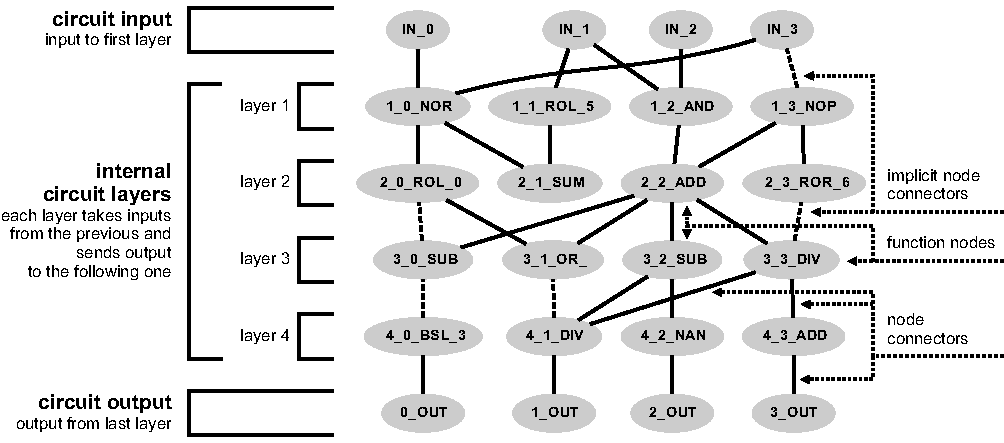
\includegraphics[scale=0.8]{./img/circuit-final.pdf}
	\caption{Vizualizáciu obvodu z {bakalárskej práce}~\parencite{ukrop-bc} Martina Ukropa.}
	\label{obr:circuit-example}
\end{figure}

Celý priebeh algoritmu spočíva v nasledujúcich krokoch:\vspace{-10pt}
\begin{enumerate}
	\item \textbf{Náhodné vygenerovanie obvodov}\\Vytvorí sa tzv. populácia náhodných jedincov. Veľa z nich bude neúspešných, avšak nájdu sa aj takí, ktorí budú od ostatných lepší. 
	\item \textbf{Určenie úspešnosti}\\Úspešnosť sa vypočíta pomocou tzv. funkcie vhodnosti, ktorá je pre správny priebeh veľmi dôležitá.
	\item \textbf{Vyradenie neúspešných obvodov}
	\item \textbf{Sexuálne skríženie najúspešnejších jedincov}\\Skrížením dostaneme novú populáciu jedincov. Cieľom kríženia je dosiahnuť novú silnejšiu generáciu, založenú len na tých najlepších jedincoch z predchádzajúcej populácie.
	\item \textbf{Náhodná mutácia niektorých jedincov}\\Aby sa zabránilo zaseknutiu sa v lokálnom maxime, je potrebné urobiť nejakú náhodnú mutáciu, napríklad odobrať cestu, alebo zmeniť niektorý z uzlov. Mutácia prebieha tak, že sa postupne prechádza obvodom a pri každom uzle respektíve hrane sa z nejakou pravdepodobnosťou vykoná mutácia.
	\item Kroky 2-5 su prevádzané v cykle až kým sa nedosiahne požadovaná úspešnosť alebo kým sa nevyčerpá určený počet generácií.
\end{enumerate}
Podstata genetiky je nájsť obvod, ktorý vie rozlišovať medzi naozaj náhodnými dátami a skúmanými dátami. Ak sa takýto obvod nájde, znamená to, že EACirc objavil v skúmaných dátach niečo, čo sa v naozaj náhodných dátach vyskytuje zriedkavo. To znamená, že dáta zrejme nebudú náhodné.

\section{Typy uzlov}
\label{sec:nodes}

V tejto sekcii si vysvetlíme aká je vlastne podstata samotného fungovania obvodov. Ako už bolo spomenuté v \hyperref[sec:genetics]{sekcii 2.2} každý jedinec sa skladá z horizontálnych vrstiev, kde v každej vrstve sa nachádzajú uzly. Každý uzol nesie v sebe informáciu, uloženú na 4 Bytoch, kde na prvom byte je uložené číslo funkcie ktorá sa má vykonať. Na ostatných miestach sú potom uložené voliteľné parametre. Avšak nie všetky funkcie tieto parametre využívajú. Jedná sa o nasledujúce funkcie:

\begin{myItemize}
	\item \textbf{Bitové operátory}\\AND, OR, XOR, NOR, NAND, ROTL, ROTR, BITSELECTOR
	\item \textbf{Aritmetické funkcie}\\SUM, SUBS, ADD, MULT, DIV
	\item \textbf{Operátor identity}\\NOP
	\item \textbf{Operátor na priame čítanie zo vstupu}\\READX
\end{myItemize}
Prvá vrstva je vstupná, to znamená, že sa do nej nalejú dáta. Následne dáta prebublávajú smerom nadol, každý uzol dostane na vstupe výstup z niekoľkých uzlov z predchádzajúcej vrstvy, vykoná funkciu, ktorej referenciu má v sebe uloženú a výstup pošle ďalšiemu respektíve ďalším uzlom v nasledujúcej vrstve. 

Použitím jednoduchých funkcií sa dá v konečnom dôsledku docieliť podobnému testu ako sa vyskytuje v štatistických testoch (\hyperref[chap:statistic-tests]{kapitola 1.}). Avšak použitie genetického algoritmu prináša aj možnosť vymyslieť lepšie a silnejšie testy ako sa nachádzajú v batériách. Preto je našim úmyslom vytvoriť pre genetiku čo najlepšiu situáciu na skonštruovanie výsledného obvodu. Následkom je myšlienka, nepoužívať v uzloch iba jednoduché funkcie (napríklad AND, OR atď.), ale vykonať v uzle niečo zložitejšie, napríklad inštrukcie vybraté z programu, ktorý vygeneroval testovaný prúd dát (viac v \hyperref[chap:eacirc-jvmsim]{kapitole 3.}).

\section{Interpretácia výsledkov}
\label{sec:result-interpretation}

EACirc má pre každý beh hypotézu, či sú skúmané dáta náhodné alebo nie. Na konci behu sa táto hypotéza buď potvrdzuje alebo zamieta. Ak sa hypotéza potvrdí, znamená to, že dáta sú náhodné, ak nie, tak EACirc našiel obvod, ktorý vie rozlíšiť medzi skúmanými a náhodnými dátami. To či sa hypotéza zamietne alebo potvrdí sa rozhoduje podľa p-value, čo je hodnota, ktorá je výsledkom každého behu, a hladiny významnosti, čo je hodnota špecifikovaná v konfiguračnom súbore a určuje ktorá je najväčšia hodnota, pre ktorú sa hypotéza ešte zamieta. To znamená, že po získaní p-value sa táto hodnota porovná s hladinou významnosti, ak je p-value menšia, hypotéza sa zamieta, inak sa potvrdzuje. 

Keďže celý algoritmus je náhodný a nie vždy sa musí genetike podariť zostrojiť úspešný obvod, existuje istá pravdepodobnosť, takisto ako pri štatistických testoch, že EACirc aj náhodné dáta označí za nenáhodné a naopak. Preto sa výpočty vždy počítajú na viac behov, vždy s náhodným semienkom. Výsledok takýchto výpočtov bude tzv. proportion, čo znamená pomer pre nás úspešných behov ku všetkým behom, teda percentuálne zastúpenie takýchto behov. Pre nás úspešné behy sú také, v ktorých bol EACirc úspešný v hľadaní obvodu, to znamená v ktorých bola hypotéza zamietnutá. Ak je proportion menšia ako hladina významnosti, väčšinou 5\%, znamená to, že EACirc nebol úspešný v hľadaní obvodu a teda skúmané dáta sú náhodné. Čím vyššie číslo proportion tým vo viac behoch bol EACirc úspešný v hľadaní obvodu. 



